\documentclass[main.tex]{subfiles}
\begin{document}
\section{Введение} \label{intro}

Одним из наиболее распространённых способов анализа генетических особенностей организмов является исследование \textit{однонуклеотидных полиморфизмов} (далее ОНП) (англ. single-nucleotide polymorphism, SNP). ОНП определяется как замена одного нуклеотида в выравнивании последовательности ДНК конкретного организма относительно некоторого генома, эталонного для данной популяции, но не любая, а только такая, которая встречается у статистически значимой доли особей в популяции \cite{butler}.\\
Полиморфизмы встречаются как в генах, так и в некодирующих областях ДНК и могут быть классифицированы по значимости, то есть по степени влияния на фенотип организма. Данные об ОНП для одного индивидуума позволяют определить принадлежность к той или иной популяции, а также судить о его отличии от среднего в популяции; данные об ОНП двух организмов дают возможность составить представление об их относительном различии. Данные о полиморфизмах большой выборки индивидуумов можно использовать для филогенетического анализа. \\
Число однонуклеотидных полиморфизмов, которые могут встретиться в одном организме, зачастую превышает несколько тысяч, поэтому для интерпретации собранных в эксперименте данных удобно пользоваться средствами визуализации, например, с помощью методов сокращения размерности проецировать точки в двух- или трёхмерное пространство. В настоящей работе на примере данных об ОНП в геномах 929 людей, которые были взяты из открытого источника, рассматривается методик визуализации, основанных на расчёте матрицы расстояний между всеми геномами. Проведено сравнение ряда метрик, используемых для составления матрицы.

\newpage
\section{Исходные данные} \label{input}

Исследуемые данные -- набор информации об ОНП в геноме человека, находящиеся в свободном доступе в базе данных Ensembl (\href{https://www.ensembl.org}{ensembl.org}). База содержит большое число записей, поэтому решено было ограничиться частью: выбраны случайным образом данные о девяноста тысячах полиморфизмов и соответствующие данные об их наличии в 928 геномах (примерно 20 000 000 записей в формате [ID человека] - [ID мутации] - [число встреч (1 -- только в одной хромосоме из диплоидного набора, 2 -- в обеих)]).

\section{Описание методик} \label{alg_desc}

\subsection{Способы вычисления расстояния}\label{section:metrics}

Для каждого экземпляра генетического материала известно, какие виды полиморфизмов из заданного набора присутствуют и какова аллельность мутации: мутации нет (0), мутация есть в одной хромосоме (1) или в обеих (2). Были составлены матрицы попарных расстояний между векторами признаков, где каждый признак соответствует своему ОНП и принимает значенияе 0, 1 или 2; каждый вектор соответствует индивидууму.

В простейшем случае расстояние между геномами принимается равным расстоянию Хэмминга, то есть
\begin{equation}\label{eq:hamming}
    dist_1(g^{(1)}, g^{(2)}) = \sum_{i} | g^{(1)}_i - g^{(2)}_i |
\end{equation}
(расстояние между наборами ОНП $g^{(1)}$ и $g^{(2)}$ вычисляется как сумма модулей разности значений аллельностей).

Также были программно реализованы и применены к данным три другие формулы, которые учитывают особенности предметной области векторов:

\begin{itemize}
    \item Расстояние с учётом высокой значимости мутации в обеих аллелях: известно, что, если мутация произошла в обеих хромосомах, то ей следует придавать существенно большее значение, чем мутации в какой-либо одной из хромосом. Поэтому можно перед расчётом расстояния преобразовать исходный вектор данных, подкорректировав значения аллельности: $0 \to 0$ (если нет мутации, значение признака нулевое); $ 1 \to 0.3 $ (мутация в одной аллели даёт вклад $0.3$); $ 2 \to 1.0 $ (мутация в обеих аллелях). Значения весов подобраны экспериментально \cite{ensembl}.  После подобного преобразования применяется расстояние Хэмминга:
    \begin{equation}\label{eq:allele}
        dist_2(g^{(1)}, g^{(2)}) = \sum_{i} | w(g^{(1)}_i) - w(g^{(2)}_i) |
    \end{equation}
    Здесь функция $w$ -- описанное выше преобразование аллельности в вес.

    \item Расстояние с учётом серьёзности последствий мутации: в базе данных Ensembl предоставлены аннотации к полиморфизмам (не к каждому, но здесь рассмотрены только полиморфизмы с аннотациями). Аннотация включает такую характеристику, как серьёзность мутации (Impact), которая может принимать одно из четырёх значений: "high"\hspace{0pt} (мутация в белок-кодирующей области, приводящая, вероятно, к потере полезной функции белка), "moderate"\hspace{0pt} (мутация в белок-кодирующей области, которая, возможно, влечёт за собой эффективность работы белка), "low"\hspace{0pt} (мутация в белок-кодирующей области, которая, скорее всего, не будет оказывать заметного влияния на функционирование фермента), и "modifier"\hspace{0pt} (мутация в некодирующей области). \\
    Имея аннотации, можно придать вес каждому признаку в общей сумме при подсчёте попарного расстояния. Тогда формула имеет вид:
    \begin{equation}\label{eq:impact}
        dist_3(g^{(1)}, g^{(2)}) = \sum_{i} | g^{(1)}_i - g^{(2)}_i | \cdot Impact_i
    \end{equation}
    Здесь $ Impact_i = 1 $ соответствует значению "high"\hspace{0pt}, $ 0.3 $ -- "moderate"\hspace{0pt}, $ 0.1 $ -- "low"\hspace{0pt}, $ 0.01 $ -- "modifier"\hspace{0pt}. Значения, как и в предшествующем пункте, подобраны экспериментально.

    \item Наконец, можно соединить методики, описанные в предыдущих пунктах, и получить расстояние с учётом веса аллельности и последствий мутаций:
    \begin{equation}\label{eq:impact_allele}
        dist_4(g^{(1)}, g^{(2)}) = \sum_{i} | w(g^{(1)}_i) - w(g^{(2)}_i) | \cdot Impact_i
    \end{equation}


\end{itemize}

\subsection{Методы визуализации}\label{section:viz}

В работе были использованы четыре метода визуализации: три из них основаны на матрице расстояний (тепловая карта, филогенетическое дерево, взвешенный граф); четвёртый (t-SNE) работает непосредственно с векторами признаков (значений аллельности ОНП).

\subsubsection{Тепловая карта}

Один из наиболее простых и общеупотребимых методов визуализации расстояний матрицы расстояний -- тепловая карта. Столбцы и строки проходят сортировку, в результате которой более близкие по значениям попарных расстояний столбцы оказываются ближе друг к другу; каждому значению расстояния ставится в соответствие цвет (в данном случае малым расстояниям соответствуют тёмно-красные клетки, большим -- светло-жёлтые). Результат для матриц, построенных по значимым ОНП для каждой из четырёх метрик, размещён в приложении (рис. \ref{fig:heatmap_manh} -- \ref{fig:heatmap_impact_allele}).


\subsubsection{Дерево Neighbour-Joining}

Один из распространённых способов компактного графического представления массива геномных данных заключается в построении филогенетического дерева, которое не только отражает близость точек, но и может указать, насколько давно предположительно произошла дивергенция между группами.

Метод соединения ближайших соседей работает с матрицей расстояний. Это пошаговый алгоритм, который строит дерево, начиная с листьев: на каждой итерации соединяет два соседних узла, то есть удалят их из дерева и добавляет новый узел, вычисляя расстояния от него до остальных узлов по формуле

$$ \rho_{km} = \frac{1}{2} (\rho_{im} + \rho_{jm} - \rho_{ij}) \thickspace \forall k $$

где $i$, $j$ -- соединяемые узлы, $m$ -- новый узел.\\

Алгоритм Neighbour-Joining хорошо зарекомендовал себя на практике при построении филогенетических деревьев \cite{durbin}, потому и был применён в данной работе. \\

Подобное филогенетические дерево строится в предположении того, что длины рёбер \textit{аддитивны}: расстояние между двумя узлами дерева равняется сумме длин рёбер на пути от одного узла к другому. Можно заметить, что все четыре функции расстояния проходят <<тест на аддивность>> -- выполняется \textit{условие четырёх точек} (four-point condition): для любых четырёх геномов $ i, j, k, l $ два расстояния из трёх $ \rho_{ij} + \rho_{kl}, \rho_{ik} + \rho_{jl}, \rho_{il} + \rho_{jk} $ не меньше, чем третье (это следует из неравенства треугольника).

\subsubsection{Взвешенный граф} \label{section:viz:graph}

Помимо прочего, в работе рассмотрен эвристический метод визуализации с помощью взвешенного графа. Для этого по матрице расстояний строится полный граф, где узлы соответствуют индивидуумам и веса рёбер -- попарным расстояниям. Затем вершины располагаются в форме окружности так, что ближайшие вершины находятся рядом. После этого можно, убрав из графа рёбра с большим весом, посмотреть, какие вершины остались связанными с соседними (рис. \ref{fig:graphs_0_5}-\ref{fig:graphs_100}).

\begin{figure}[H]
    \centering
    \begin{subfigure}{.3\textwidth}
        \centering
        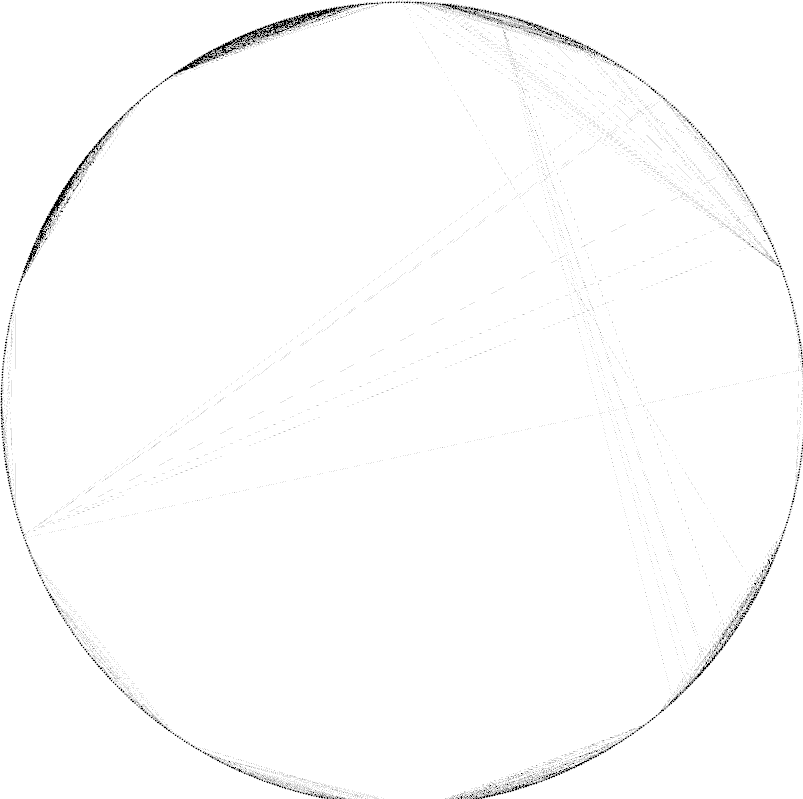
\includegraphics[width=\linewidth]{significant/graphs_examp/mh_impact_0_5percent}
        \captionsetup{width=.8\linewidth}
        \caption{0.5\% рёбер}
        \label{fig:graphs_0_5}
    \end{subfigure}%
    \begin{subfigure}{.3\textwidth}
        \centering
        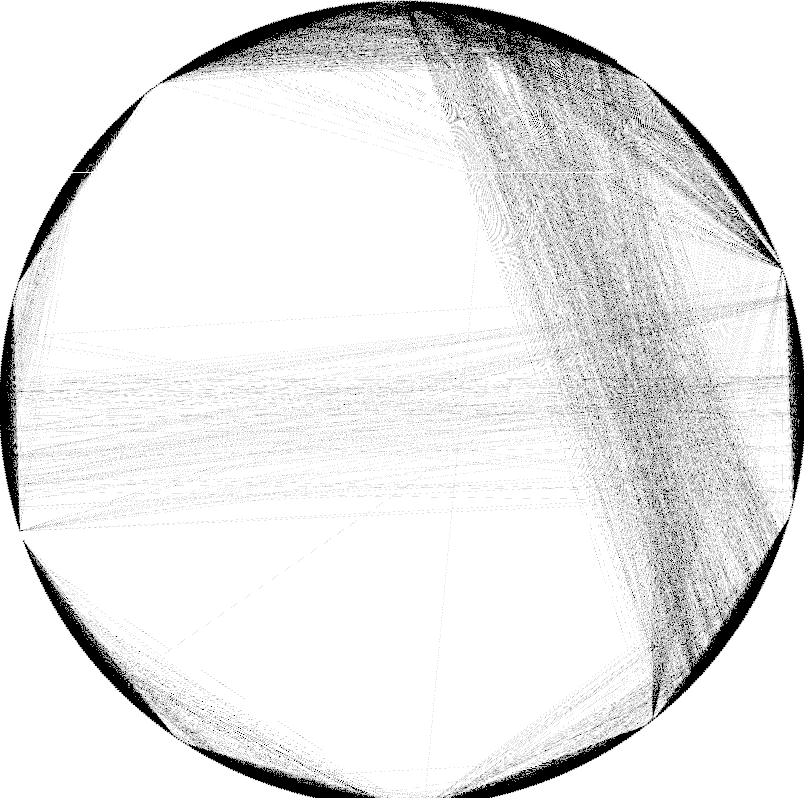
\includegraphics[width=\linewidth]{significant/graphs_examp/mh_impact_6percent}
        \captionsetup{width=.8\linewidth}
        \caption{6\% рёбер}
    \end{subfigure}%
    \begin{subfigure}{.3\textwidth}
        \centering
        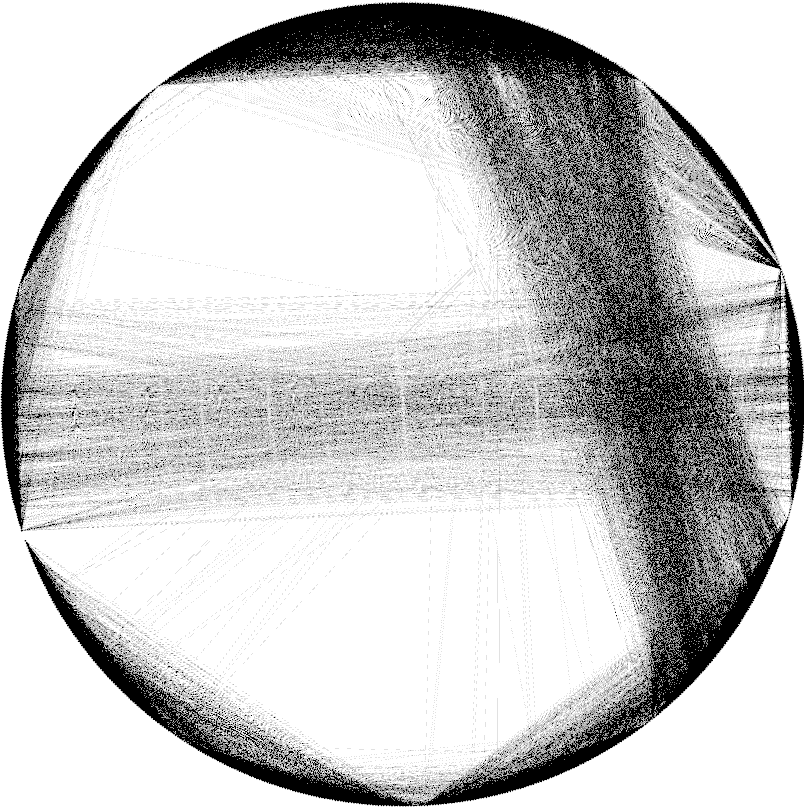
\includegraphics[width=\linewidth]{significant/graphs_examp/mh_impact_10percent}
        \captionsetup{width=.8\linewidth}
        \caption{10\% рёбер}
    \end{subfigure}

    \begin{subfigure}{.3\textwidth}
        \centering
        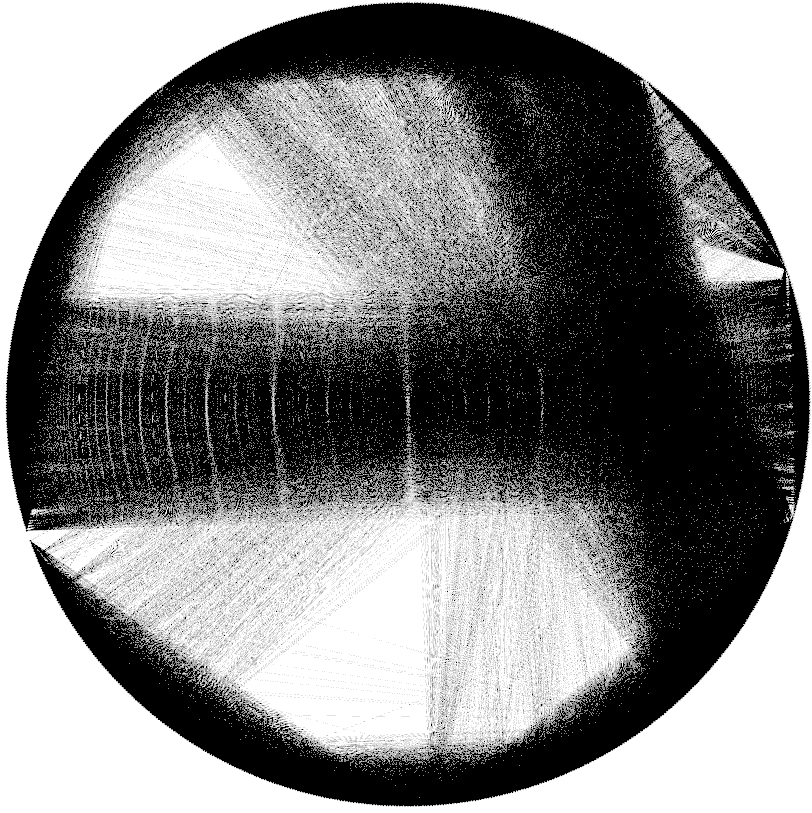
\includegraphics[width=\linewidth]{significant/graphs_examp/mh_impact_17percent}
        \captionsetup{width=.8\linewidth}
        \caption{17\% рёбер}
    \end{subfigure}%
    \begin{subfigure}{.3\textwidth}
        \centering
        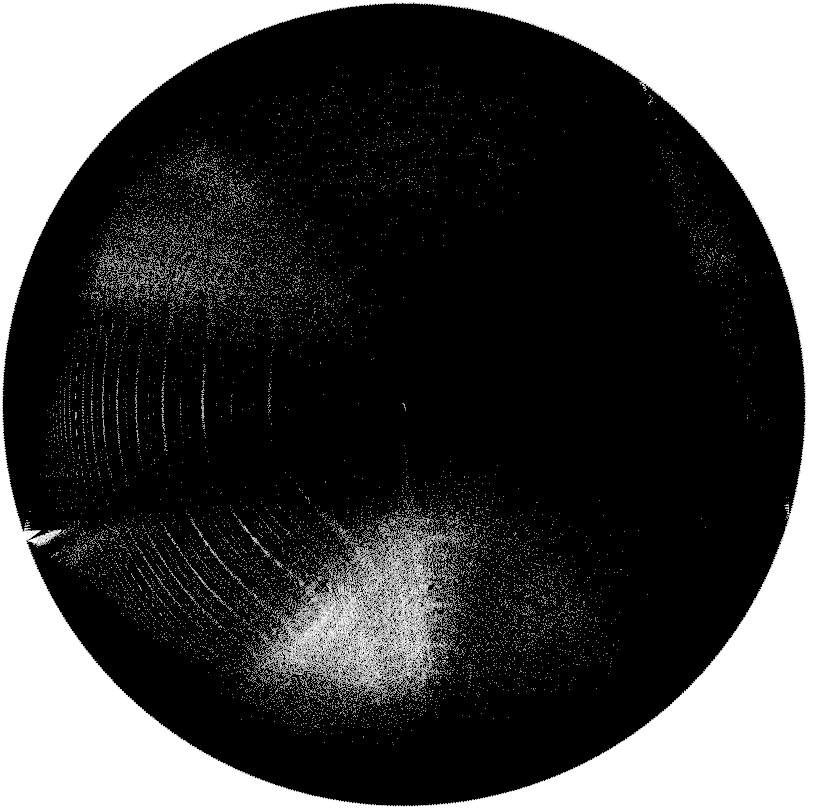
\includegraphics[width=\linewidth]{significant/graphs_examp/mh_impact_30percent}
        \captionsetup{width=.8\linewidth}
        \caption{30\% рёбер}
    \end{subfigure}%
    \begin{subfigure}{.3\textwidth}
        \centering
        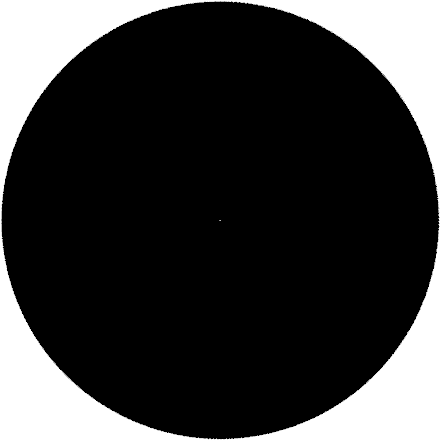
\includegraphics[width=\linewidth]{significant/graphs_examp/mh_impact_100percent}
        \captionsetup{width=.8\linewidth}
        \caption{100\% рёбер}
        \label{fig:graphs_100}
    \end{subfigure}
    \caption{Граф, построенный по матрице смежности. Показаны только рёбра с самым низким весом.}
\end{figure}


\subsubsection{t-SNE}

t-SNE (t-Distributed Stochastic Neighbor Embedding) -- алгоритм сокращения размерности данных, который стремится сохранить близость между точками, исходя из их вероятности быть соседями. Этот метод часто используется для визуализации, поскольку его отличительная особенность -- за счёт использования распределения Стьюдента для расчёта вероятностей соседства точек данные в пространстве низкой размерности не собираются, в отличие от других методов, в одну группу (что позволяет визуально выделять на изображениях кластеры) \cite{tsne}. \\
В данной работе метод был использован как верификация прочих, то есть сравнивается число кластеров, полученных методом t-SNE, с числами, полученными иными способами.

\section{Проведённые эксперименты}\label{experiments}

Составлены (и затем запущены на множестве исходных данных) программы на языке Python, реализующие методы, описанные в разделе \ref{section:viz}. Построение тепловых карт, дерева расстояний и t-SNE уже заложены в библиотеках, поэтому их несложно было применить к данным; основная часть проделанной работы заключается в манипуляциях с большими объёмами данных (исходный набор включает более 20 миллионов записей). Для эффективной работы с этими значениями создан конвейер, включающий множество однотипных шагов, каждый из которых принимает на вход один или несколько файлов и записывает один или несколько файлов. Таким образом, при необходимости прерванную по каким-либо причинам работу программы можно восстановить без необходимости проводить заново все операции. \\
На первой ступени конвейер считывает информацию о полиморфизмах, записанную в форме двух таблиц -- соответствие ID опытного образца идентификатору ОНП с указанием аллельности этого SNP (1 или 2) и соответствие ID ОНП степени влияния (impact) (подробно об impact см. раздел \ref{section:metrics}). Эта информация используется для составления векторов признаков для каждого опытного образца. Как отмечалось в разделе \ref{section:metrics}, не все полиморфизмы имеют аннотации, поэтому вектор признаков имеют меньшую длину, чем число различных полиморфизмов (признаки без аннотаций отбрасываются). Далее строятся матрицы расстояний и на их основе производится визуализация. \\
Кроме того, составленные матрицы расстояний в формате csv были использованы для построения графов (см. \ref{section:viz:graph}) с помощью пакета Gephi. \\

В результате из множества данных по SNP получены четыре набора изображений, соответствующие расстояниям, рассчитанным по формулам \eqref{eq:hamming}, \eqref{eq:allele}, \eqref{eq:impact} и \eqref{eq:impact_allele}: тепловые карты (рисунки \ref{fig:heatmap_manh} - \ref{fig:heatmap_impact_allele}), деревья (рис. \ref{fig:nj_manh} - \ref{fig:nj_impact_allele}) и графы (рис. \ref{fig:signif_manhattan_graph} - \ref{fig:signif_impact_allele_graph}).
Здесь приведены изображения графов, на которых сохранён $1\%$ от общего числа рёбер; вообще говоря, как было выяснено на практике, удаётся получить правдоподобную картинку при сохранении $0.5-15\%$ рёбер. \\
Также векторы признаков были обработаны алгоритмом t-SNE, реализованном в Python-библиотеке scikit-learn. Результаты приведены на рис. \ref{fig:signif_tsne_2d} (сокращение до двух измерений) и \ref{fig:signif_tsne_3d} (три измерения). Также для сравнения алгоритм был запущен на наборе векторов без фильтрации признаков, то есть в случае, когда в признаках присутствуют в том числе и ОНП без аннотации (рис. \ref{fig:all_tsne_2d} и \ref{fig:all_tsne_3d}). \\

Исходный код программ доступен по адресу: \href{https://github.com/zuevval/snp-visualizer}{github.com/zuevval/snp-visualizer}

\newpage

\section{Анализ результатов}
Метод t-SNE при сокращении размерности до двух даёт набор точек, в которых ясно можно различить десять обособленных кластеров. Это верно как для векторов признаков исключительно с аннотациями, так и для <<полного>> множества признаков, причём при сокращении признаков точки лучше группируются в кластеры.
Такой результат позволяет предположить, что фильтрация признаков по наличию аннотации позволяет оставить только значимые ОНП; возможно, впрочем, что при рассмотрении СНП без аннотации можно было бы среди найденных десяти кластеров выделить близкие, но всё же отдельные подгруппы. Во всяком случае, в первом приближении фильтрация ОНП не приводит к потере информации о кластерах.\\
Визуализация в трёхмерном пространстве не даёт результатов, которым можно придать подобную интерпретацию, что является общим местом для t-SNE: как правило, он даёт более наглядное изображение на плоскости \cite{tsne}. \\

Глядя на тепловую карту и дерево Neighbour-Joining, полученные по матрице расстояний Хэмминга (рис. \ref{fig:heatmap_manh} и \ref{fig:nj_manh}), можно увидеть те же десять кластеров. Следовательно, подобное представление имеет смысл: близость в пространстве признаков отражается в матрице.
Надо отметить, впрочем, что добавление в метрику поправок, связанных с учётом значимости и аллельности, по-видимому, не даёт преимущества: кластеры, напротив, размываются, становятся менее выраженными, появляются выбросы. На рис. \ref{fig:hist_manh} - \ref{fig:hist_impact_allele} показаны диаграммы распределения значений элементов в матрицах расстояний; видно, что при добавлении поправок большая часть элементов сосредотачивается в области малых значений, то есть наблюдается тенденция к сближению точек в одну общую группу, что для нас плохо. \\

Метод визуализации при помощи графа является эвристическим и нет гарантии того, что конфигурация рёбер и вершин соответствуют существующим в действительности связям между геномами. Несмотря на это, такой способ представления оказывается удобным: все остальные методы дают <<статическую>> картинку, в то время как граф легко изменить, задавая порог фильтрации рёбер, и таким образом добиться ожидаемого числа кластеров на изображении. Для каждой из четырёх формул расстояния при сохранении $1\%$ самых <<лёгких>> рёбер можно, как и при визуализациях иными методами, выделить десять кластеров (рис. \ref{fig:signif_manhattan_graph} - \ref{fig:signif_impact_allele_graph}).

\section{Заключение}

В работе рассмотрены три метода визуализации набора данных об ОНП в геномах, основанные на расчёте матрицы попарных расстояний, и один, основанный на сокращении размерности.
Каждый из них можно использовать для графического представления массива данных. Проведены попытки улучшить качество представления с помощью корректировки формулы расстояния путём добавления поправок, вводимых из соображений, определяемых предметной областью; но подобные техники не дали заметного улучшения результата.

В качестве продолжения работы можно к данным в исходной размерности или к точкам, полученным в результате применения t-SNE, применить какой-либо алгоритм кластеризации (например, метод $k$ средних с параметром $k=10$), после чего посмотреть, как распределены точки из этих кластеров на тепловой карте, в иерархической структуре дерева и на диаграмме взвешенного графа.
Также можно провести все те же расчёты для большего набора данных (как было отмечено в разделе \ref{input}, в данной работе используется лишь около $1\%$ данных об ОНП в геномах, хранящихся в базе Ensembl).

\end{document}
